\documentclass[20 pts]{article}
\usepackage{xeCJK}
\usepackage{amsfonts}
\usepackage{amssymb}
\usepackage{amsmath}
\usepackage{bm}
\setCJKmainfont{SimSun}
\title{プログラミング言語基礎論第2回レポート} 
\author{Kwame Ackah Bohulu, 1631133}
\date{21-08-2017}
\begin{document}
\maketitle

\newpage

\paragraph{[1-a]}
--Built-inFunctions\\
builtinFns :: [([Char], [Char])]\\
builtinFns = [("square", "lambda x . x * x"),\\
              ("fourthPower", "lambda x . square (square x)"),\\
              ("abs","lambda x . if x < 0 then (0 - x) else x")]\\
              
              
\paragraph{[1-b]}

ToEnv :: [([Char], [Char])] ->[(Variable, Val)]\\
ToEnv [] =[]\\
ToEnv ((k,v):ps) = (k,vv) : ToEnv ps\\
                          where vv = ev v\\

globalEnv :: Env \\
globalEnv = ToEnv builtinFns\\

\paragraph{[1-c]}
ev :: [Char] -> Val\\
ev s = expval (parseProg s) globalEnv

\begin {center}
\begin{figure}[h!]
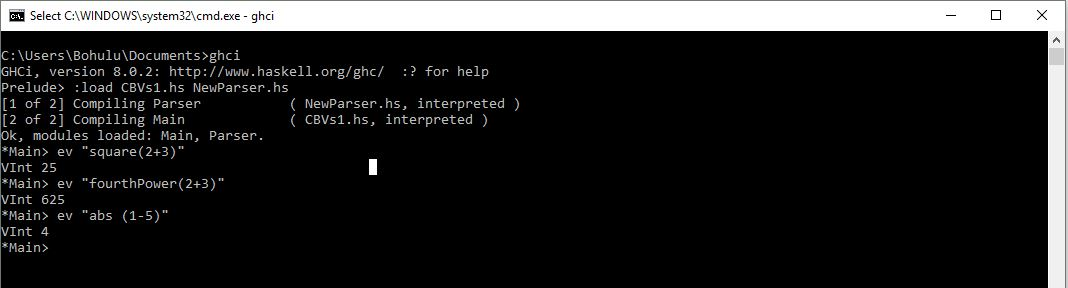
\includegraphics[width=8cm]{1_b.jpg}
\label{SystemModel}
\end{figure}
\end{center}


    \newpage   
    \paragraph{[2-1]}
     5行目から14行目の部分を次のように 変更\\
     
     data Val = VInt Int\\
         | VBool Bool\\
         | VClosure Variable Expr Env Bool\\
         deriving (Eq, Show)\\

showVal :: Val -> [Char]\\
showVal (VInt m) = show m\\
showVal (VBool b) = show b\\
showVal (VClosure v e r b) =\\
  "Closure [lambda " ++(if b then "@" else "")++ show v ++ " . " ++ show e ++ "]"
  \paragraph{}
        72行目から78行目の部分を次のように 変更\\
        expval (Fun x e) env = VClosure x e env True\\

expval (SFun x e) env = VClosure x e env False\\

expval (Apply e1 e2) env =
  v `seq` g `seq` expval body newenv\\
  where g = expval e1 env\\
        v = ( if t then delay e2 env  else Evaled (expval e2 env))\\
        VClosure x body env' t = g\\
        newenv = updateEnv x v env'\\
        
        \begin {center}
\begin{figure}[h!]
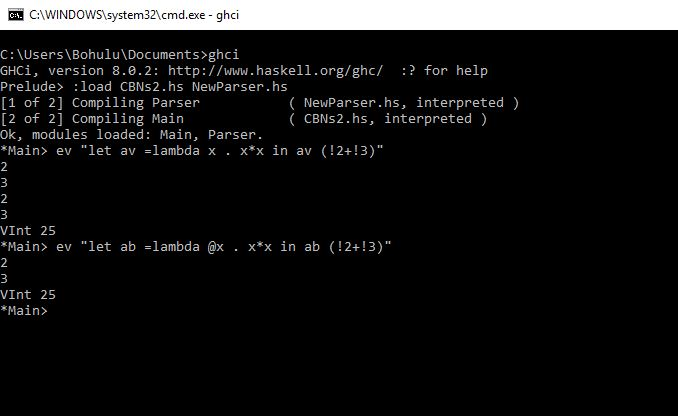
\includegraphics[width=8cm]{2_1.jpg}
\label{SystemModel}
\end{figure}
\end{center}
       


\end{document}